% Sample file for 'CACM - Research Highlights'-type articles
% Created by: Gerry Murray, Elec. Pub. Info. Mgr., Pubs. Dept., ACM HQ, NY.
% (murray@hq.acm.org)
%
% This is "research-highlights-sample.tex" (sample file) V1.1 Sept. 2008
% This file should be compiled with V1.1 of "research4cacm.cls" Sept. 2008
%
% If you have already submitted an article to an ACM/SIGS Conference, and have had your
% article published in one of the 'Proceedings', then you have probably used
% the (ACM/SIGS) 'sig-alternate' class and .tex file.
% Any such 'conference-prepared' source .tex file is 'compatible' with the class file
% 'research4cacm' which you will use to prepare your article for inclusion in the magazine 'CACM'.
%
% Here are the steps to take in order to 'morph' your article from being
% a 'conference' article to one more suitable for inclusion in 'Communications of the ACM'.
%
% 1. Change \documentclass{sig-alternate}  to \documentclass{research4cacm}
%
% 2. Comment out the conference information e.g.  %\conferenceinfo{WOODSTOCK}{'97 El Paso, Texas USA}
%
% 3. Make sure the copyright data is correct e.g. \crdata{0001-0782/08/0200}
%
% 4. Make sure the YEAR is correct e.g. \CopyrightYear{2008} with the current default being �2008�.
%
% 5. Comment out the Classification scheme, general terms and keywords.
%
% 6. If you have mentioned authors in the 'Additional Authors' section you should
%    'move them back' into the byline (so that they appear with all the other authors).
%    ALL authors, in Research Highlights articles, get equal billing.
%
% 7. Suitably edit the file (i.e. body text) so as to make it more appropriate for a wider audience.
%
% If, early on in the editorial process, the 'correct' copyright data becomes available
% please change the copyright data to suit, otherwise leave the default '0001-0782/08/0X00'.
% (The editorial staff will change it later on in the production cycle.)
%
% ================= IF YOU HAVE QUESTIONS =======================
% Technical questions _only_ to
% Gerald Murray (murray@hq.acm.org)
% ===============================================================
% ---------------------------------------------------------------------------------------------------------------
%
\documentclass{research4cacm}

\usepackage{graphicx, subfigure, multirow, times, balance}
\usepackage{balance, url, amsfonts, verbatim, mathtools, algpseudocode, algorithm}

\newcommand{\commentt}[1]{{\small\texttt{#1}}}
\renewcommand{\ttdefault}{cmtt}

\newtheorem{definition}{Definition}

\sloppy

\newcommand{\sectionskip}{-0em}
\newcommand{\subsectionskip}{-0em}
\newenvironment{myitemize}
{
   \vspace{0mm}
    \begin{list}{$\bullet$ }{}
        \setlength{\topsep}{0em}
        \setlength{\parskip}{0pt}
        \setlength{\partopsep}{0pt}
        \setlength{\parsep}{0pt}         
        \setlength{\itemsep}{1mm} 
}
{
    \end{list} 
    \vspace{-1em}
}

\begin{document}
%
% --- Author Metadata here ---
% Conference information is NOT appropriate for CACM so comment it out.
%\CopyrightYear{2008} % Allows default copyright year (2008) to be over-ridden - IF NEED BE.
%\crdata{0001-0782/08/0X00}  % Allows default copyright data (0001-0782/08/0X00) to be over-ridden - IF NEED BE.
% --- End of Author Metadata ---

\title{Quantifying Eventual Consistency with PBS}
% \titlenote{(This is a simple titlenote.)For use with research4cacm.cls. Supported by ACM.}
%
% Show use of \thanks - which can appear here (normal/default) or down by the author
\thanks{The original version of this paper is entitled
  ``Probabilistically Bounded Staleness for Practical Partial Quorums"
  and was published in VLDB 2012~\protect\cite{pbs-vldb}. An invited extended
  version of this paper is entitled ``Quantifying Eventual Consistency
  with PBS'' and will appear in the VLDB Journal's ``Best of VLDB
  2012'' issue in 2014~\protect\cite{pbs-vldbj}. Portions of this work also
  appear in a SIGMOD 2013 demo entitled ``PBS at Work: Advancing Data
  Management with Consistency Metrics''~\protect\cite{pbs-sigmod}.}

%\titlenote{A full version of this paper is available in...}
%
% You need the command \numberofauthors to handle the 'placement
% and alignment' of the authors beneath the title.
%
% For aesthetic reasons, we recommend 'three authors at a time'
% i.e. three 'name/affiliation blocks' be placed beneath the title.
%
% NOTE: You are NOT restricted in how many 'rows' of
% "name/affiliations" may appear. We just ask that you restrict
% the number of 'columns' to three.
%
% Use the \alignauthor commands to handle the names
% and affiliations.
%
\numberofauthors{1} %  in this sample file, there are a *total*
% of SIX authors and all of them fit neatly on the first page.
% As said, all authors get 'equal billing' and you should fit all of them on the opening page
% in the 'byline'. The production/editorial-staff will 'separate' names from their affiliations, leaving
% author names beneath the title (in the byline), and moving the affilations/contact information to an area
% after the references at the back of the article.
%
% You can go ahead and credit any number of authors here,
% e.g. one 'row of three' or two rows (consisting of one row of three
% and a second row of one, two or three).
%
% The command \alignauthor (no curly braces needed) should
% precede each author name, affiliation/snail-mail address and
% e-mail address. Additionally, tag each line of
% affiliation/address with \affaddr, and tag the
% e-mail address with \email.
%
% 1st. author
\author{Peter Bailis, Shivaram Venkataraman, Michael J. Franklin, Joseph M. Hellerstein, Ion Stoica\\
\affaddr{University of California, Berkeley}\\
\affaddr{\{pbailis, shivaram, franklin, hellerstein, istoica\}@cs.berkeley.edu}}
\maketitle



\begin{abstract}

Data replication results in a fundamental trade-off between operation
latency and consistency. At the weak end of the spectrum of possible
consistency models is eventual consistency, which provides no limit to
the staleness of data returned. However, anecdotally, eventual
consistency is often ``good enough'' for practitioners given its
latency and availability benefits. In this work, we explain this
phenomenon and demonstrate that, despite their weak guarantees,
eventually consistent systems regularly return consistent data while
providing lower latency than their strongly consistent
counterparts. To quantify the behavior of eventually consistent
stores, we introduce Probabilistically Bounded Staleness (PBS), a
consistency model that provides expected bounds on data staleness with
respect to both versions and wall clock time. We derive a closed-form
solution for versioned staleness and model real-time staleness for a
large class of quorum replicated, Dynamo-style stores. Using PBS, we
measure the trade-off between latency and consistency for partial,
non-overlapping quorum systems under Internet production workloads. We
quantitatively demonstrate how and why eventually consistent systems
frequently return consistent data within tens of milliseconds while
offering large latency benefits.
%, where it currently ships as a feature of the software distribution.

\end{abstract}


\vspace{\sectionskip}\section{Introduction}

Modern distributed data stores need to be scalable, highly available,
and fast. These systems typically replicate data across different
machines and increasingly across datacenters for at least two reasons:
first, to provide availability when components fail and, second, to
provide improved performance by serving requests from multiple
replicas. Configuring and maintaining replicated data has significant
consequences for application and data store
design~\cite{abadilatconsist}. Performance at scale is critical for a
large class of applications and, in practice, increased latencies may
correspond to large amounts of lost revenue~\cite{perf-impact}. For
example, at Amazon, 100~ms of additional latency resulted in a 1\%
drop in sales~\cite{amazon-latency}, while 500~ms of additional
latency in Google's search resulted in a corresponding 20\% decrease
in traffic~\cite{google-talk}. However, lowering latency in
distributed data stores has a cost: contacting fewer replicas for each
operation can adversely impact achievable semantic guarantees.

To provide predictably low latency, modern systems often eschew
protocols guaranteeing ``strong'' consistency of reads (e.g., the
illusion of a single-copy of replicated data) and instead opt for
``weaker'' semantics, frequently in the form of \textit{eventual
  consistency}~\cite{abadilatconsist,pbs-vldb,pbs-vldbj,dynamo}.  This
eventual consistency is one of the weakest properties provided by
modern stores: it provides no guarantees on data staleness except
that, in the absence of new writes, reads will ``eventually'' return
the effect of the most recent write(s)~\cite{vogels-defs}. Under this
definition, a store that returns data that is weeks old is eventually
consistent, as is a store that returns arbitrary data (e.g., always
return value 42) as long as, at \textit{some point} in the future, the
store returns the last written data~\cite{eventual-queue}. Due to this
near-absence of useful semantics for end users, the decision to employ
eventual consistency is often
controversial~\cite{hamilton-cap,walter,urbanmyths}. In the many
production stores providing eventual consistency
today~\cite{dynamo,riaktalkone}, users have little to no insight into
the behavior of their stores or the consistency of their data,
especially under varying replication configurations.  However, the
proliferation of eventually consistent deployments suggests that
applications can often tolerate occasional staleness and that data
tends to be ``fresh enough'' in many cases.

In this work, we bridge this gap between theoretical guarantees and
current practice by quantifying the degree to which eventual
consistency is both eventual and (in)consistent and explain
why. Indeed, under worst-case conditions, eventual consistency results
in an unbounded degree of data staleness. However, as we will show,
the common case is often different. Core to our thesis is the
observation that eventual consistency can be modeled as providing a
probabilistic \textit{expectation} of consistency given a particular
workload and deployment environment. Accordingly, for varying degrees
of certainty, eventually consistent stores can offer bounds on how far
they may deviate from strongly consistent behavior. We present
probabilistic models for such bounds called Probabilistically Bounded
Staleness, or PBS.
% certainty, can offer staleness bounds with respect to time (``how
% eventual'') and versions (``how consistent''). 
% We present probabilistic answers to these questions, which we call
% Probabilistically Bounded Staleness, or PBS.

To predict consistency with PBS, we need to know when and why eventually
consistent systems return stale data and how to quantify the staleness
of the data they return.  In this paper, we present algorithms and
models for two common staleness metrics in the literature: wall clock
time~\cite{rahman2012toward} and versions~\cite{vahdat-article}.  PBS
describes both measures, providing the probability of reading a write
$\Delta$ seconds after the write returns ($(\Delta, p)$-semantics, or ``how
eventual is eventual consistency?''), of reading one of the last $K$
versions of a data item ($(K, p)$-semantics, or ``how consistent is
eventual consistency?''), and of experiencing a combination of the two
($(K, \Delta, p)$-semantics). PBS does not propose new mechanisms to
enforce deterministic staleness bounds~\cite{vahdat-article}; instead,
our goal is to provide a lens for analyzing, improving, and predicting
the behavior of \textit{existing}, widely deployed systems.

In this work, we apply PBS to quorum-replicated data stores such as
Dynamo~\cite{dynamo} and its several open source descendants. Quorum
systems ensure strong consistency across reads and writes to replicas
by ensuring that read and write replica sets overlap. However,
employing \textit{partial} (or non-strict) quorums can lower latency
by requiring fewer replicas to respond.  With partial quorums, sets of
replicas written to and read from need not overlap: given $N$ replicas
and read and write quorum sizes $R$ and $W,$ partial quorums imply
$R$$+$$W$$\leq$$N$. For partial quorums we derive closed-form
solutions for PBS $(K, p)$-regular semantics and use Monte Carlo
methods to explore the trade-off between latency and $(\Delta,
p)$-regular semantics.

%We expand prior work on 
%\textit{probabilistic quorums}~\cite{prob-quorum,quorum-overview} to account for
%multi-version staleness and messaging protocols as used in today's
%systems. 

%Using production latency distributions, 
%
%PBS $(\Delta, p)$-regular semantics.

Finally, we use PBS to study the staleness observed in production
deployments of Dynamo-style data stores under normal operation (i.e.,
failure-free scenarios). We show how high variance in write latency
can lead to an increased window of inconsistency.  For example, in one
production environment, switching from spinning disks to solid-state
drives dramatically improved consistency (e.g., $1.85$ms versus
$45.5$ms wait time for a $99.9$\% probability of consistent reads) due
to decreased write latency mean and variance.  We also make
quantitative observations of the latency-consistency trade-offs
offered by partial quorums.  For example, in another production
environment, we observe an $81.1\%$ combined read and write latency
improvement at the $99.9$th percentile ($230$ to $43.3$ms) for a
$202$ms window of inconsistency ($99.9\%$ probability consistent
reads). This analysis helps demonstrate the performance benefits that
lead operators to choose eventual consistency and motivates additional
end-user applications ranging from consistency monitoring to
consistency-based SLAs and query planning.

\section{Probabilistically Bounded Staleness}
\label{sec:pbs-defs}

By popular definitions, eventually consistent data stores do not make
any guarantees as to the recency of data that they return: ``if no new
updates are made to the object, eventually all accesses will return
the last updated value''~\cite{vogels-defs}. This is a useful
\textit{liveness} property, guaranteeing that something good
eventually happens, but it provides no \textit{safety} properties: the
data store can return any data in the
interim~\cite{eventual-queue}. Many real-world eventually consistent
stores do not make any guarantees beyond this definition, yet they are
widely deployed and have seen increased popularity over the past
decade (Section~\ref{sec:practice}).  As we will see, the protocols
used by most eventually consistent stores indeed do not
\textit{enforce} additional guarantees, but they may \textit{supply}
them during operation.

%To account for non-guaranteed but usually-provided semantics, in this paper,
To quantify semantics that are not guaranteed but are often provided,
we develop a probabilistic framework for reasoning about consistency,
called Probabilistically Bounded Staleness, or PBS. There are a wide
range of possible consistency models that a data store can provide,
from linearizability to causal consistency to eventual consistency;
what is the likelihood that an end user will observe a given
consistency model if it is not guaranteed? Here, we study variants of
two classic kinds of (in)consistency in the form of staleness:
versions and time. We develop variants of PBS metrics that provide
quantitative expectations that a store will return a version that was
written within the last $K$ writes of the latest (where $K=1$ is
latest) and that a store will return the latest version as of $\Delta$
seconds ago. Ultimately this does \textit{not} provide a guarantee,
but it is still useful for reasoning about and introspecting the
behavior of a given system, similar to the usage of modern
service-level agreements (SLAs) on performance
(Section~\ref{sec:discussion}).

To begin, we first need to define a baseline for ``strongly
consistent'' semantics. The Dynamo-style stores we study provide a
choice between ``strong'' \textit{regular} semantics and eventual
consistency; we subsequently observe when the eventually consistent
choices behave like their ``strong'' counterparts. According to the
distributed systems literature~\cite{non-strict}:

\begin{definition}
A read from a given data item obeys {\normalfont{regular semantics}}
if, in the case that the read does not overlap (in real time)
with any writes to the same item, it returns the result the last
completed write, or, if the read overlaps (in real time) with at least
one write to the same data item, it returns either the result of the
last completed write or the eventual result of one of the overlapping
writes.
\end{definition}

Accordingly, regular semantics provide the illusion of a single copy
of each replicated data item, except when there are concurrent reads
and writes, during which writes' effects may become visible and
subsequently ``disappear.'' While this special, overlapping case is
somewhat awkward to reason about (cf. definitions of
linearizability~\cite{linearizability}), this is a widely deployed
data replication configuration.

Before we consider PBS applied to regular semantics, we first present
a generalization of the semantics to account for for multi-version
staleness~\cite{non-strict}:

\begin{definition}
A read from a given data item obeys {\normalfont{$K$-regular
    semantics}} if, in the case that the read does not overlap
(in real time) with a write to the same data item, it returns the
result of one of the latest $K$ completed writes, or, if the read
overlaps (in real time) with a write to the same item, it returns
either the result of one of the latest $K$ completed writes or the
eventual result of one of the overlapping writes.
\end{definition}

$K$-regular semantics are useful for reasoning about
\textit{how stale} a given read can be and can also be used to enforce
additional consistency properies such as monotonic reads, where
reads do not appear to ``go back in time''~\cite{pbs-vldb, sessionguarantees}.

We now present our first application of PBS principles. Given a
system that does not guarantee $K$-regular semantics, we can reason
about its semantics by taking a probabilistic approach:

\begin{definition}
A system provides {\normalfont{$(K, p)$-regular semantics}} if each read
provides $K$-regular semantics with probability $p$.
\end{definition}

This modification is simple and straightforward: given an existing
semantic guarantee, we can consider a probabilistic version of it,
whereby reads may or may not obey the property. Of course, the above
is simply a definition, and we must still determine how to actually
provide PBS predictions, which will be the focus of the rest of the
paper.

In addition to considering version-based staleness, we can also
consider staleness with respect to real time. As we will see, message
propagation and processing delays can influence consistency across
time, so we extend regular semantics to consider time as well:

\begin{definition}
A read obeys {\normalfont{$\Delta$-regular semantics}} if it returns
either the result of the latest write as of up to $\Delta$ time units
ago, the result of a write that was started but not completed as of up
to $\Delta$ time units ago, or the eventual result of any of currently
overlapping writes.
\end{definition}

We can similarly extend this definition to a probabilistic context:

\begin{definition}
A system provides {\normalfont{$(\Delta, p)$-regular semantics}} if each read obeys
$\Delta$-regular semantics with probability $p$.
\end{definition}

Although we do not consider them in this article, it is possible to
consider both time and version staleness together, which we term $(K,
\Delta, p)$ staleness semantics~\cite{pbs-vldb,pbs-vldbj}.

\vspace{\sectionskip}\section{Quorum System Background}
\label{sec:background}

With PBS metrics in hand, we can proceed to apply them to real
systems, where they are most useful. In this study, we will consider
PBS metrics in the context of quorum-replicated data stores, which
represent a large class of widely deployed real-world distributed data
stores. However, with some work, we believe that our methodology is
also applicable to other styles of replication. Here, we provide
background on quorum systems, with a focus on current practice.

\vspace{\subsectionskip}\subsection{Quorum Foundations: Theory}

Quorum systems have a long tradition as a replication strategy for
distributed data~\cite{quorum-overview}.  Under quorum replication, a
data store writes a data item by sending it to a set of servers
responsible for the (\textit{replicas}), called a write quorum.  To
serve reads, the data store fetches the data from a possibly different
set of replicas, called a read quorum.  For reads, the data store
compares the set of values returned by the replicas, and, given a
total ordering of versions, can return the most recent value (or all
values received, if desired).  For each operation, the data store
chooses (read or write) quorums from a set of sets of replicas, called
a \textit{quorum system}, with one system per data item.  There are
many kinds of quorum systems, but one simple configuration is to use
read and write quorums of fixed sizes, which we will denote $R$ and
$W$, for a set of replicas of size $N$. A \textit{strict quorum
  system} has the property that any two quorums in the quorum system
overlap (have non-empty intersection), providing regular semantics.  A
simple example of a strict quorum system is the majority quorum
system, in which each quorum is of size $\lceil
\frac{N+1}{2}\rceil$. \textit{Partial quorum systems}, which we will
study, are a natural relaxation of strict quorum systems: at least two
quorums in a partial quorum system do not overlap~\cite{prob-quorum}.

% There are two relevant variants of partial quorum
% systems described in the literature: probabilistic quorum systems and
% k-quorums.

%\textit{Probabilistic quorum systems} provide probabilistic guarantees
%of quorum intersection.  By scaling the number of replicas, one can
%achieve an arbitrarily high probability of
%consistency~\cite{prob-quorum}.  Intuitively, this is a consequence of
%the Birthday Paradox: as the number of replicas increases, the
%probability of non-intersection between any two quorums decreases. As
%an example, consider $N$ replicas with randomly chosen read and write
%quorums of sizes $R$ and $W$. We can calculate the probability that
%the read quorum does not contain the last written version. This
%probability is the number of quorums of size $R$ composed of nodes
%that were not written to in the write quorum divided by the number of
%possible read quorums:
%\begin{equation}
%\label{eq:prob-strict}
%p_{s}=\frac{{N-W \choose R}}{{N \choose R}}
%\end{equation}
%The probability of inconsistency is high except for large $N$.  With
%$N=100$, $R=W=30$, $p_{s} = 1.88 \times
%10^{-6}$~\cite{non-strict}.  However, with $N=3$, $R=W=1$, $p_{s}
%= 0.\overline{6}$.  The asymptotics of these systems are
%excellent---but only at asymptotic scales.

%\textit{$k$-quorum systems} provide \textit{deterministic} guarantees
%that a partial quorum system will return values that are within $k$
%versions of the most recent write~\cite{non-strict}.  In a single
%writer scenario, sending each write to $\lceil\frac{N}{k}\rceil$
%replicas with round-robin write scheduling ensures that any replica is
%no more than $k$ versions out-of-date.  However, with multiple
%writers, we lose the global ordering properties that the single-writer
%was able to control, and the best-known algorithm for the pathological
%case results in a lower bound of $(2N-1)(k-1)+N$ versions
%staleness~\cite{multi-k-quorum}.

\vspace{\subsectionskip}\subsection{Quorum Foundations: Practice}
\label{sec:practice}

In practice, many distributed data management systems use quorums as a
replication mechanism. Amazon's Dynamo~\cite{dynamo} is the progenitor
of a class of eventually consistent data stores that include Apache
Cassandra\footnote{\url{http://cassandra.apache.org/}}, Basho
Riak\footnote{\url{http://www.basho.com/riak/}}, and Project
Voldemort\footnote{\url{http://www.project-voldemort.com/}}.  All of
these systems use the same variant of quorum-style replication and we
are not aware of any widely adopted data store using a vastly
different quorum replication protocol. 

Dynamo-style quorum systems employ one quorum system per data item,
typically maintaining the mapping of items to quorum systems using a
consistent-hashing scheme or a centralized membership protocol. Each
server in the system cluster stores multiple items.  As shown in
Figure~\ref{fig:dynamo-quorum}, clients send read and write requests
to a server in the system cluster, which subsequently forwards the
request to \textit{all} replicas for the operation's item.  This
coordinating server considers an operation complete when it has
received responses from a pre-determined number of replicas (typically
configured per-operation).  Accordingly, without message loss, all
replicas eventually receive all writes. Dynamo denotes the replication
factor of an item as $N$, the number of replica responses required for
a successful read as $R$, and the number of replica acknowledgments
required for a successful write as $W$. Like other strict quorum
systems, Dynamo provides regular semantics when $R$$+$$W$$>$$N$ during
failure-free operation. However, unlike traditional quorum systems,
Dynamo's write quorum size increases even after the operation returns,
growing via \textit{anti-entropy}~\cite{eventual-queue,dynamo}.
Coordinators send all requests to all replicas but consider only the
first $R$ ($W$) responses.  As a matter of nomenclature (and to
disambiguate against ``dynamic'' quorum membership protocols), we will
refer to these systems as \textit{expanding partial quorum systems}.

\begin{figure}
\centering
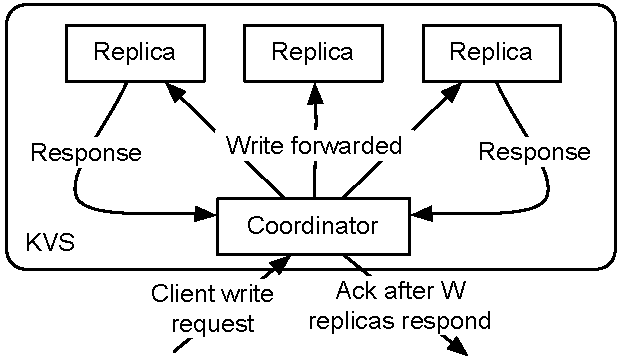
\includegraphics[width=.85\columnwidth]{figs/dynamo-quorum.pdf}
\caption{Diagram of control flow for client write to Dynamo-style
  quorum ($N=3$, $W=2$).  A coordinator server handles the client write
  and sends it to all $N$ replicas. The write call returns after the
  coordinator receives $W$ acknowledgments.}
\label{fig:dynamo-quorum}
\end{figure}

As we discuss in extended versions of this
paper~\cite{pbs-vldb,pbs-vldbj}, system operators often report using partial
quorum configurations in Dynamo-style stores, citing ``maximum
performance'' in the ``general case,'' particularly for ``low value''
data or queries that need ``very low latency and high availability.''


\vspace{\sectionskip}\section{PBS and Partial Quorums}
\label{sec:pbs-quorum}

Given our PBS metrics and an understanding of quorum behavior, we can
develop models for the probability of consistency under partial
quorums. Here, we briefly discuss version-based staleness for
traditional probabilistic quorums and develop a more complex
``white box'' model of time-based staleness for Dyanamo-style systems.

\vspace{\subsectionskip}\subsection{PBS $(K, p)$-regular semantics}
\label{sec:kstale}

To understand static, non-expanding quorum behavior, we first revisit
probabilistic quorum systems~\cite{prob-quorum}, which provide
probabilistic guarantees of quorum intersection in partial quorum
systems. As an example, consider $N$ replicas with read and write
quorums of sizes $R$ and $W$ chosen uniformly at random. We can
calculate the probability that the read quorum does not contain the
last written version. This probability is the number of quorums of
size $R$ composed of replicas that were not written to in the write
quorum divided by the number of possible read quorums:
\begin{equation}
\label{eq:prob-strict}
p_{s}=\frac{{N-W \choose R}}{{N \choose R}}
\end{equation}

The probability of inconsistency is high for small values of $N$.
However, by scaling the number of replicas and quorum sizes, one can
achieve an arbitrarily high probability of
consistency~\cite{prob-quorum}.  For example, with $N=3$, $R=W=1$,
$p_{s} = 0.\overline{6}$, but with $N=100$, $R=W=30$, $p_{s} = 1.88
\times 10^{-6}$~\cite{non-strict}.  This is reminiscent of the
Birthday Paradox: as the number of replicas increases, the probability
of non-intersection between any two quorums decreases. Hence, the
asymptotics of these systems are excellent---but only at asymptotic
scales.

While probabilistic quorums allow us to determine the probability of
returning the most recent value written to the database they do not
describe what happens when the most recent value is not returned.
Here, we determine the probability of returning a value within a
bounded number of versions ($(K,p)$-regular semantics).  In the
following formulation, we consider traditional, non-expanding write
quorums (no anti-entropy).

Similar to the previous example, given independent, identically
distributed (IID) choice of read and write quorums, returning one of
the last $k$ written versions is equivalent to intersecting one of $k$
independent write quorums.  Given the probability of a single quorum
non-intersection $p$, the probability of non-intersection with one of
the last $k$ independent quorums is $p^k$. Thus, the probability of
non-intersection with uniform random choice in our example quorum
system is Equation \ref{eq:prob-strict} exponentiated by $k$:
\begin{equation}
\label{eq:k-consistency}
p = \left(\frac{{N-W \choose R}}{{N \choose R}}\right)^k
\end{equation}

When $N$$=$$3$, $R$$=$$W$$=$$1$, this means that the probability of
returning a version within $2$ versions is $0.\overline{5}$, within $3$
versions, $0.\overline{703}$, $5$ versions, $> 0.868$, and $10$
versions, $>0.98$.  When $N$$=$$3$, $R$$=$$1$, $W$$=$$2$ (or, equivalently,
$R$$=$$2$, $W$$=$$1$), these probabilities increase: $k$$=$$1
\rightarrow 0.\overline{6}$, $k$$=$$2 \rightarrow 0.\overline{8}$, and
$k$$=$$5 \rightarrow > 0.995$.

This closed form solution holds for quorums that do not change size
over time.  For expanding partial quorum systems, this solution is a
lower bound on $p$ for $(K, p)$-regular semantics. In the full version
of this paper, we consider more advanced formulations of this
analysis, including an analysis of monotonic reads consistency, quorum
load, and closed-form solutions for mixed time and
versions~\cite{pbs-vldb,pbs-vldbj}.

\vspace{\sectionskip}\subsection{Consistency in Dynamo}
\label{sec:dynamo}

We have a simple, closed-form model for $(K, p)$-regular semantics,
but time-based ($(\Delta, p)$-regular) semantics are dependent on the
quorum replication algorithm, workload, and any anti-entropy processes
employed by a given system.  In this section, we develop techniques
for analyzing PBS $(\Delta, p)$-regular semantics in the context of
Dynamo-style data stores.

Dynamo-style quorum systems are inconsistent as a result of read and
write message reordering, in turn a product of message delays. In this
work, we take a white box approach to inconsistency and directly
examine the protocols behind consistency. Accordingly, we develop a
model of message latency in Dynamo operation that captures the effects
of message delays for write requests (\texttt{W}), write
acknowledgments (\texttt{A}), read requests (\texttt{R}), and read
responses (\texttt{S}), and which, for convenience, we call
\textit{WARS}. In Figure~\ref{fig:dynamo-diagram}, we illustrate
\textit{WARS} using a space-time diagram for messages between a
coordinator and a single replica for a write followed by a read
$\Delta$ seconds after the write completes.  Accordingly, $\Delta$
here corresponds to the $\Delta$ in PBS $(\Delta, p)$-regular
semantics. In brief, reads are stale when all of the first $R$
responses to the read request arrived at their replicas before the
last (completed) write request arrived.

\begin{figure}
\centering
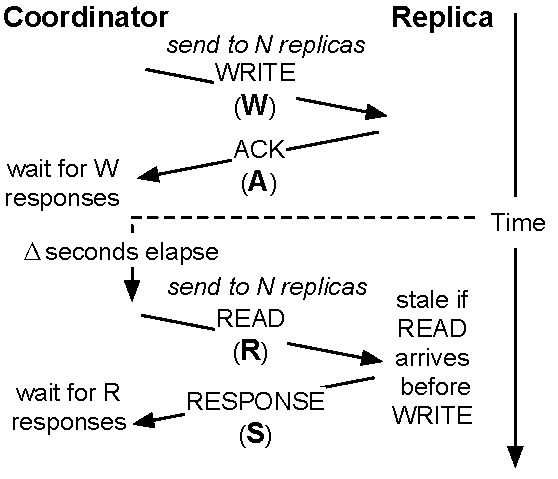
\includegraphics[width=.8\columnwidth]{figs/dynamostale.pdf}
\caption{The \textit{WARS} model describes staleness in Dynamo by
  modeling message latencies between a coordinator and replicas for a
  write operation followed by a read operation $t$ seconds later.  In
  an $N$ replica system, the pictured messages are sent $N$ times.}
\label{fig:dynamo-diagram}
\end{figure}

For a write, the coordinator sends $N$ messages, one to each
replica. The message from the coordinator to replicas containing the
write is delayed by a value drawn from distribution \texttt{W}.  The
coordinator waits for $W$ responses from the replicas before it can
consider the write completed.  Each response acknowledging the write
is delayed by a value drawn from the distribution \texttt{A}.

For a read, the coordinator (possibly different than the write's
coordinator, and possibly representing a different client than the
client that issued the write) sends $N$ messages, one to each replica.
The message from coordinator to replica containing the read request is
delayed by a value drawn from distribution \texttt{R}.  The
coordinator waits for $R$ responses from the replicas before returning
the most recent value it receives.  The read response from each
replica is delayed by a value drawn from the distribution \texttt{S}.

The read coordinator will return stale data if the first $R$ responses
received reached their replicas before the replicas received the
latest version (delayed by \texttt{W}).  When $R$$+$$W$$>$$N$, this is
impossible.  However, under partial quorums, the frequency of this
occurrence depends on the latency distributions.  If we denote the
write completion time (when the coordinator has received $W$
acknowledgments) as $w_t$, a single replica's response is stale if
$r'+w_t+\Delta< w'$ for $r'$ drawn from \texttt{R} and $w'$ drawn from
\texttt{W}.  Writes have time to propagate to additional replicas both
while the coordinator waits for all required acknowledgments
(\texttt{A}) and as replicas wait for read requests (\texttt{R}).
Read responses are further delayed in transit (\texttt{S}) back to the
read coordinator, inducing further possibility of reordering.
Qualitatively, long-tailed write distributions (\texttt{W}) and
relatively faster reads (\texttt{R},\texttt{S}) increase the chance of
staleness due to reordering.

\textit{WARS} considers the effect of message sending, delays, and
reception, but this represents a difficult analytical formulation with
several non-independent order statistics.  As we discuss in
Section~\ref{sec:mcsim}, we instead explore \textit{WARS} using Monte
Carlo methods, which are straightforward to understand and
implement. We have found that the \textit{WARS} distributions are easy
to parametrize from traces of real-world system behavior
(Section~\ref{sec:latencies}).

\vspace{\sectionskip}\section{PBS in Action}
\label{sec:dynamoeval}

Given our PBS models for Dynamo-style stores, we now apply them to
real-world systems. As discussed in Section~\ref{sec:dynamo}, PBS
$(\Delta, p)$-regular behavior in a given system depends on the
propagation of reads and writes across replicas.  We introduced the
\textit{WARS} model as a means of reasoning about inconsistency in
Dynamo-style quorum systems, but quantitative metrics such as
staleness observed in practice depend on each of \textit{WARS}'s
latency distributions.  In this section, we perform an analysis of
Dynamo-style $(\Delta, p)$-regular semantics for both synthetic and
real-world distributions to better understand how frequently
``eventually consistent'' means ``consistent'' and, more importantly,
why Dynamo-style stores are indeed frequently consistent.

PBS $(K, p)$-regular analysis for partial quorums is easily captured
in closed form (Section~\ref{sec:kstale}).  It does not depend on
write latency or any environmental variables.  Indeed, in practice,
without expanding quorums or anti-entropy, we observe that our derived
equations hold true experimentally.

In contrast, $(\Delta, p)$-regular semantics depends on anti-entropy,
which is more complicated.  In this section, we focus on deriving
experimental expectations for PBS $(\Delta, p)$-regular semantics. We
first validate our Monte Carlo analysis based on the \textit{WARS}
model and using message-level traces gathered from Cassandra clusters
in Berkeley. We next explore synthetic latency distributions and, for
the remainder of our analysis, explore distributions from two Internet
companies: LinkedIn and Yammer.

\vspace{\subsectionskip}\subsection{Monte Carlo Simulation}
\label{sec:mcsim}

We implemented \textit{WARS} analysis in a Monte Carlo-based
simulation. Calculating $(\Delta, p)$-regular semantics for a given
value of $\Delta$ is straightforward (see pseudocode
in~\cite{pbs-vldbj}). To simulate the message delays between
coordinator and each of the $N$ replicas, denote the $i$th sample
drawn from distribution \texttt{D} as $\texttt{D}[i]$ and draw $N$
samples from \texttt{W}, \texttt{A}, \texttt{R}, and \texttt{S}. 
Compute the time that the write request completes ($w_t$, or the
time that the coordinator gets its $W$th acknowledgment; the $W$th
smallest value of $\{\texttt{W}[i]+\texttt{A}[i], i \in [0, N)\}$).
Next, determine whether any of the first $R$ replicas contained an 
up-to-date response: check whether any the first $R$ samples
of \texttt{R}, ordered by $\texttt{R}[i]+\texttt{S}[i]$ obey 
$w_t+\texttt{R}[i] + \Delta\leq \texttt{W}[i]$. Repeating this process
multiple times provides a approximation of the behavior specified by 
the trace.  Extending this formulation to analyze $(K, \Delta, p)$-regular semantics given a
distribution of write arrival times will require accounting for
multiple writes across time. As described in extended versions of
this paper~\cite{pbs-vldb, pbs-vldbj}, we validated this analysis on
traces that we collected from a real-world Cassandra cluster. We
observed an average RMSE of $0.28\%$ for $(\Delta, p)$-regular
semantics prediction and an average N-RMSE of $0.48\%$ for latency
predictions.

\vspace{\subsectionskip}\subsection{Write Latency Distribution Effects}
\label{sec:synthetic}

The \textit{WARS} model of Dynamo-style systems dictates that high
variance in latency increases staleness. Before studying real-world
workloads (Section~\ref{sec:latencies}), we quantified this behavior in isolation via synthetic
distributions: we swept a range of exponentially distributed write
distributions (changing parameter $\lambda$, which dictates the mean
and tail of the distribution) while fixing
\texttt{A}=\texttt{R}=\texttt{S}.

Our results, shown in Figure~\ref{fig:varydelay}, demonstrate this
relationship.  When the variance and mean of \texttt{W} are $0.0625$
ms and $0.25ms$ ($\lambda=4$, one-fourth the mean of
\texttt{A}=\texttt{R}=\texttt{S}=$1$ ms), we observe a $94\%$ chance
of consistency immediately after the write and $99.9\%$ chance after
1ms.  However, when the variance and mean of \texttt{W} are $100$ ms
and $10$ ms ($\lambda=.1$, ten times the mean of
\texttt{A}=\texttt{R}=\texttt{S}=$1$ ms), we observe a $41\%$ chance
of consistency immediately after write and a $99.9\%$ chance of
consistency only after $65$ms.  As the variance and mean increase, so
does the probability of inconsistency.  Under distributions with fixed
means and variable variances (uniform, normal), we observe that the
mean of \texttt{W} is less important than its variance if \texttt{W}
is strictly greater than \texttt{A}=\texttt{R}=\texttt{S}.

Decreasing the mean and variance of \texttt{W} improves the
probability of consistent reads.  This means that, as we will see,
techniques that lower write latency variance result in more consistent
reads.  Instead of increasing read and write quorum sizes, operators
could chose to lower (relative) \texttt{W} latencies through hardware
configuration or by delaying reads, although this latter option is
detrimental to performance for read-dominated workloads and may
introduce undesirable queuing effects. Nonetheless, this PBS analysis
illustrates the fact that stale reads can be avoided in a variety of
ways beyond simple adjustment of quorum sizes.

\begin{figure}
\centering
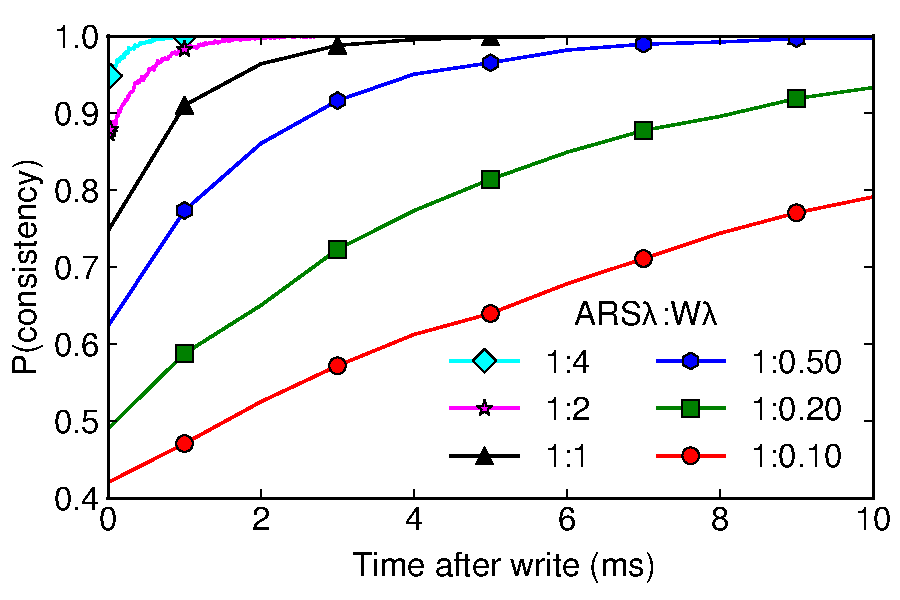
\includegraphics[width=.85\columnwidth]{figs/rwratio.pdf}
\caption{$(\Delta, p)$-regular semantics with
  exponential latency distributions for 
  \texttt{W} and \texttt{A}=\texttt{R}=\texttt{S}. Mean latency is
  $1/\lambda$. $N$$=$$3$, $R$$=$$W$$=$$1$. }
\label{fig:varydelay}
\end{figure}

\vspace{\subsectionskip}\subsection{Production Latency Distributions}
\label{sec:latencies}

To study real-world behavior, we obtained production latency
statistics from two Internet-scale companies. While message-level
\textit{WARS} timing traces would deliver more accurate predictions,
we opted for a pragmatic compromise: as described in extended versions
of this work, we fit \textit{WARS} distributions to each of the
provided statistics (Figure~\ref{fig:latencies})~\cite{pbs-vldb,
  pbs-vldbj}.

\begin{figure*}[t!]
\centering
\subfigure{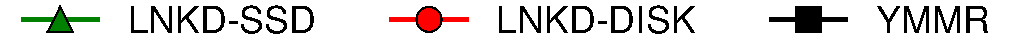
\includegraphics[width=.85\columnwidth]{figs/latlegend.pdf}}\\[-1mm]
\subfigure{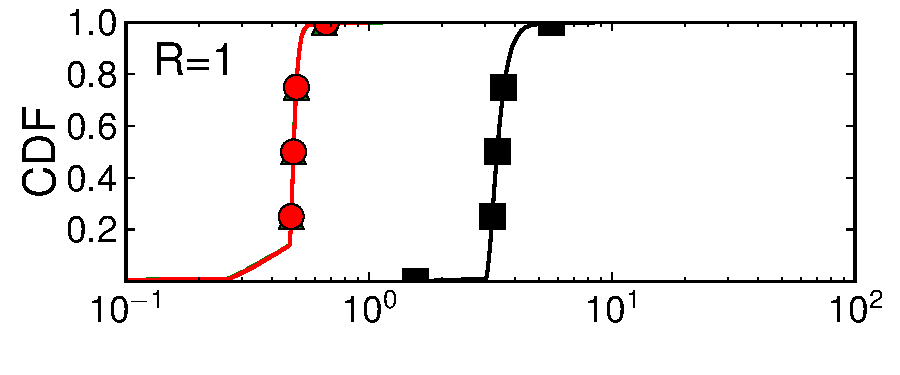
\includegraphics[width=.66\columnwidth]{figs/readlats-1.pdf}}
\subfigure{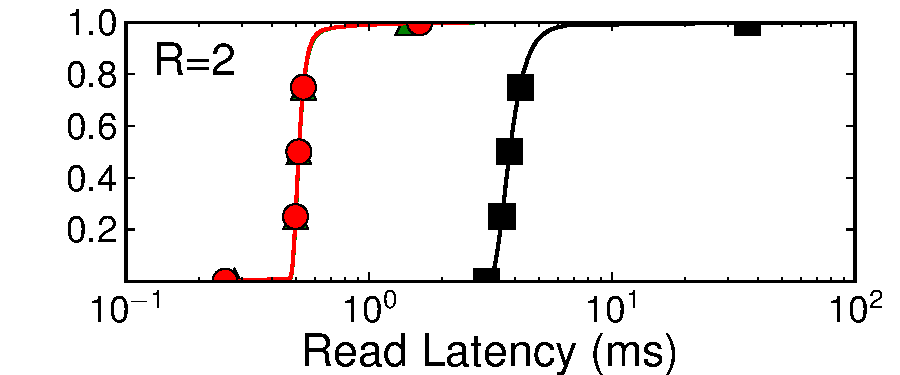
\includegraphics[width=.66\columnwidth]{figs/readlats-2.pdf}}
\subfigure{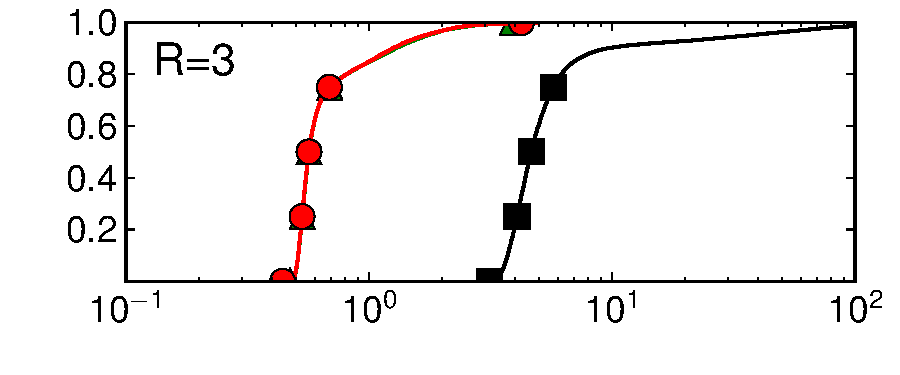
\includegraphics[width=.66\columnwidth]{figs/readlats-3.pdf}}
\subfigure{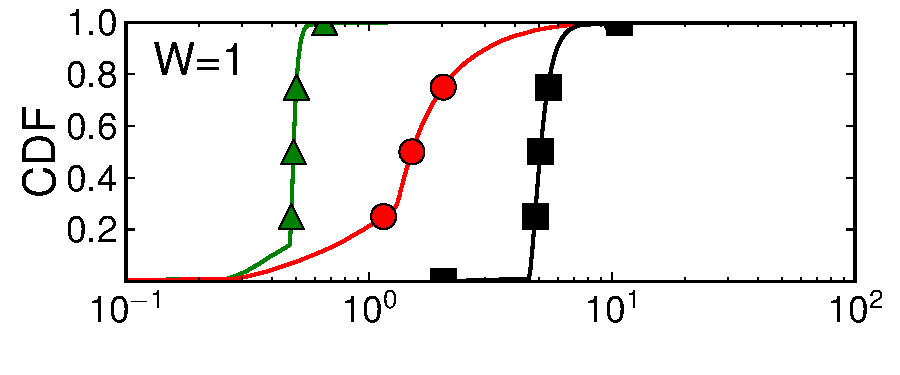
\includegraphics[width=.66\columnwidth]{figs/writelats-1.pdf}}
\subfigure{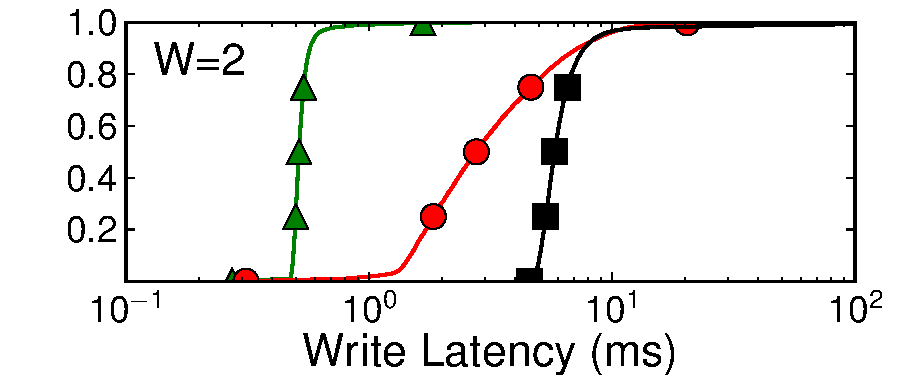
\includegraphics[width=.66\columnwidth]{figs/writelats-2.pdf}}
\subfigure{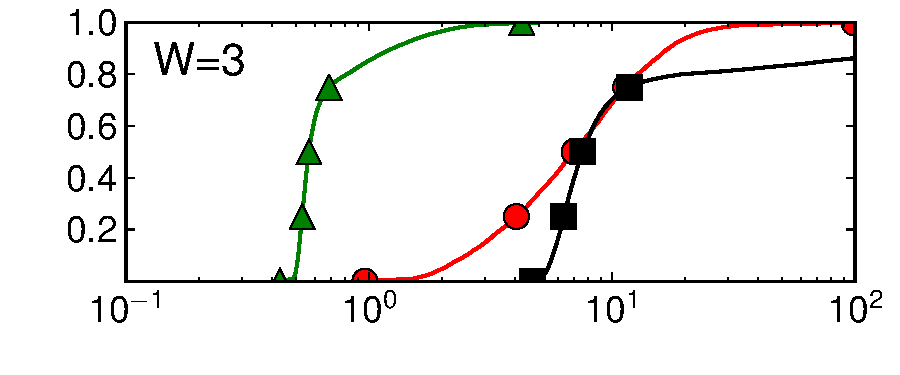
\includegraphics[width=.66\columnwidth]{figs/writelats-3.pdf}}
\caption{Read and write operation latency for production fits for
  $N$$=$$3$ and varying $R$ and $W$. For reads, \texttt{LNKD-SSD} is
  equivalent to \texttt{LNKD-DISK}. Depicted points mark significant
  percentiles for comparison. Higher values of $R$ and $W$ result in
  increased latency.}
\label{fig:latencies}
\end{figure*}

LinkedIn\footnote{\url{http://www.linkedin.com/}} is an online
professional social network with over 225 million members as of July
2013. To provide highly available, low latency data storage, engineers
at LinkedIn built Voldemort.  Alex Feinberg, a lead engineer on
Voldemort, graciously provided us with latency distributions for a
single server under peak traffic for a user-facing service at LinkedIn,
representing 60\% read and 40\% read-modify-write
traffic~\cite{pbs-vldb,pbs-vldbj}. Feinberg reports that, using
spinning disks, Voldemort is ``largely IO bound and latency is largely
determined by the kind of disks we're using, [the] data to memory
ratio and request distribution.''  With solid-state drives (SSDs),
Voldemort is often ``CPU and/or network bound'' and ``maximum latency
is generally determined by [garbage collection] activity (rare, but
happens occasionally) and is within hundreds of milliseconds.'' We
denote the LinkedIn spinning disk distribution as
\texttt{LNKD-DISK} and SSD trace as \texttt{LNKD-SSD}.

Yammer\footnote{\url{http://www.yammer.com/}} provides private social
networking to over 200,000 companies as of July 2013 and uses Basho's
Riak for some client data.  Coda Hale, an infrastructure architect,
provided us with more detailed performance statistics for their
application~\cite{pbs-vldb,pbs-vldbj}.  Hale mentioned that ``reads
and writes have radically different expected latencies, especially for
Riak.''  Riak delays writes ``until the fsync returns, so while reads
are often $<$ 1ms, writes rarely are.''  Also, although we do not
model this explicitly, Hale also noted that the size of values is
important, claiming ``a big performance improvement by adding LZF
compression to values.'' We denote the Yammer latency distribution as
\texttt{YMMR}.

%We also considered a wide-area network replication scenario, denoted
%\texttt{WAN}.  Reads and writes originate in a random datacenter, and,
%accordingly, one replica command completes quickly and the coordinator
%routes the others remotely.  We delay remote messages by 75ms and
%apply \texttt{LNKD-DISK} delays once the command reaches a remote data
%center, reflecting multi-continent WAN delay~\cite{dean-keynote}.

\vspace{\subsectionskip}\subsection{Staleness in Production}

The production latency distributions confirm that staleness is
frequently limited in eventually consistent stores. We measured the
$(\Delta, p)$-regular semantics for each distribution
(Figure~\ref{fig:tvis}). \texttt{LNKD-SSD} and \texttt{LNKD-DISK}
demonstrate the importance of write latency in practice.  Immediately
after write completion, \texttt{LNKD-SSD} had a $97.4\%$ probability
of consistent reads, reaching over a $99.999\%$ probability of
consistent reads after five milliseconds. \texttt{LNKD-SSD}'s reads
briefly raced with its writes immediately after write completion.
However, within a few milliseconds after the write, the chance of a
read arriving before the last write was nearly eliminated. The
distribution's read and write operation latencies were small (median
$.489$~ms), and writes completed quickly across all replicas due to
the distribution's short tail ($99.9$th percentile $.657$ms).  In
contrast, under \texttt{LNKD-DISK}, writes take much longer (median
$1.50$ms) and have a longer tail ($99.9$th percentile $10.47$~ms).
\texttt{LNKD-DISK}'s $(\Delta, p)$-regular semantics reflects this
difference: immediately after write completion, \texttt{LNKD-DISK} had
only a $43.9\%$ probability of consistent reads and, $10$~ms later,
only a $92.5\%$ probability.  This suggests that SSDs may greatly
improve consistency due to reduced write variance. Similarly, one
should expect that consistency would be improved by using explicit
memory management rather than unscheduled garbage collection.

We experienced similar behavior with the other distributions.
Immediately after write completion ($\Delta=0$), \texttt{YMMR} had a
$p=89.3\%$ probability of consistency.  However, the \texttt{YMMR}
distribution only reached a $p=99.9\%$ probability of consistency at
$\Delta=1364$ ms due to high variance and long-tail behavior in its
write distribution. This hints that, given multiple replicas for a
data item, the durability benefits of synchronously flushing writes to
disk may have adverse effects on consistency. An alternative approach
that could improve consistency and avoid this high variance would
relying on multi-replica (in-memory or buffer cache) replication for
durability and only flush writes asynchronously.
%As expected, \texttt{WAN} observed
%poor chances of consistency until after the 75 milliseconds passed
%($33\%$ chance immediately after commit); the client had to wait
%longer to observe the most recent write unless it originated from the
%reading client's data.

\begin{figure*}[t!]
\centering
\subfigure{
\includegraphics[width=.85\columnwidth]{figs/stalelegend.pdf}}\\[-1mm]
\subfigure{
\includegraphics[width=3.2mm]{figs/staley.pdf}}
\subfigure{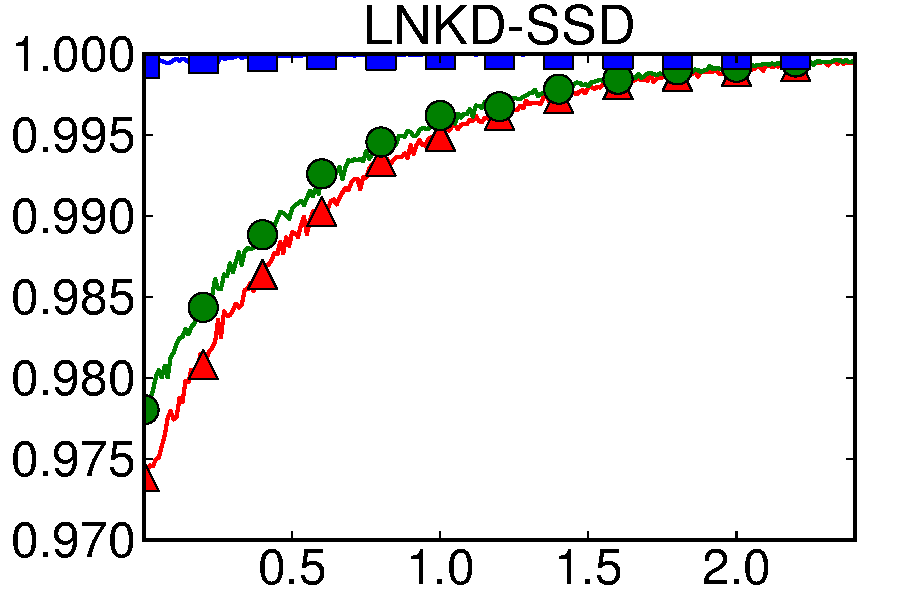
\includegraphics[width=.30\textwidth]{figs/tstales-LNKD-SSD.pdf}}
\subfigure{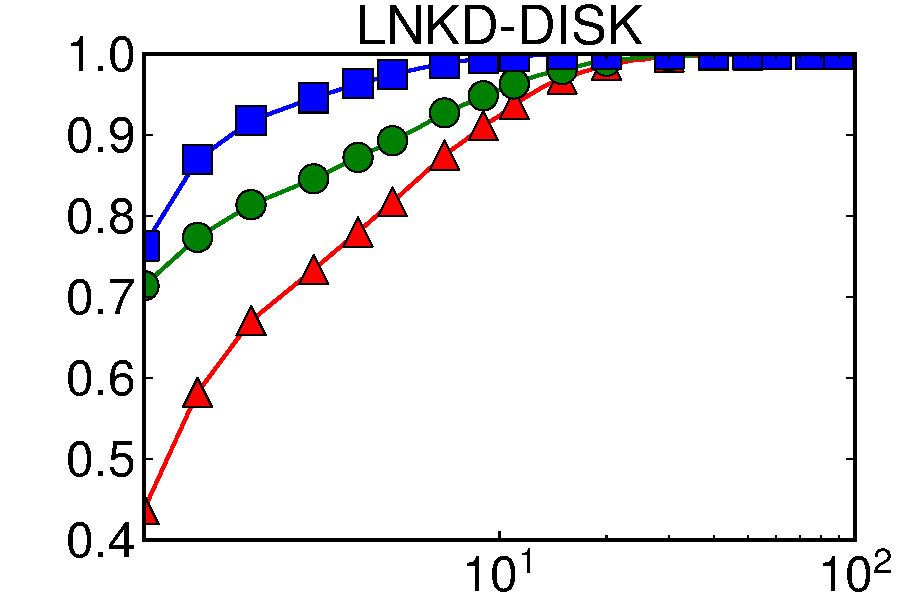
\includegraphics[width=.30\textwidth]{figs/tstales-LNKD-DISK.pdf}}
%\subfigure{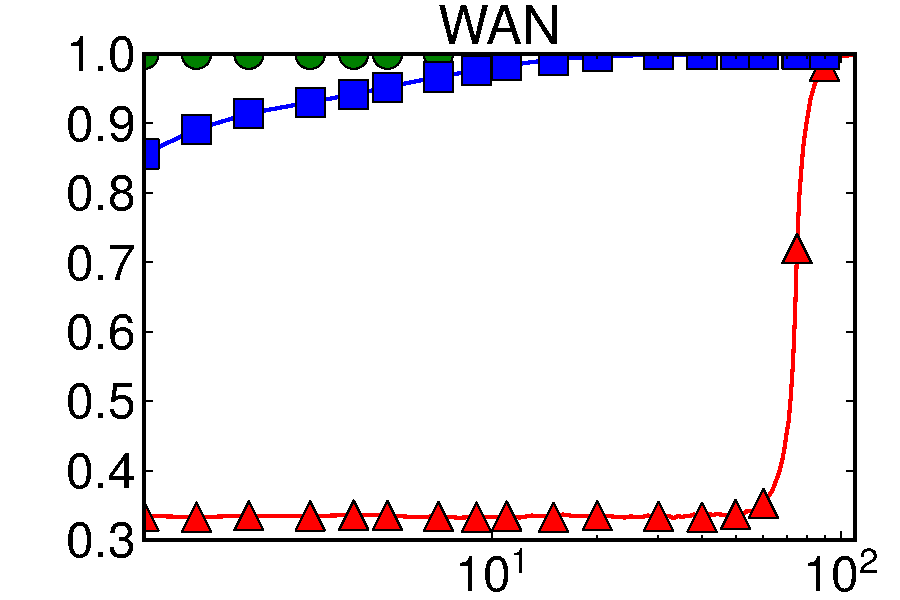
\includegraphics[width=.48\columnwidth]{figs/tstales-WAN.pdf}}
\subfigure{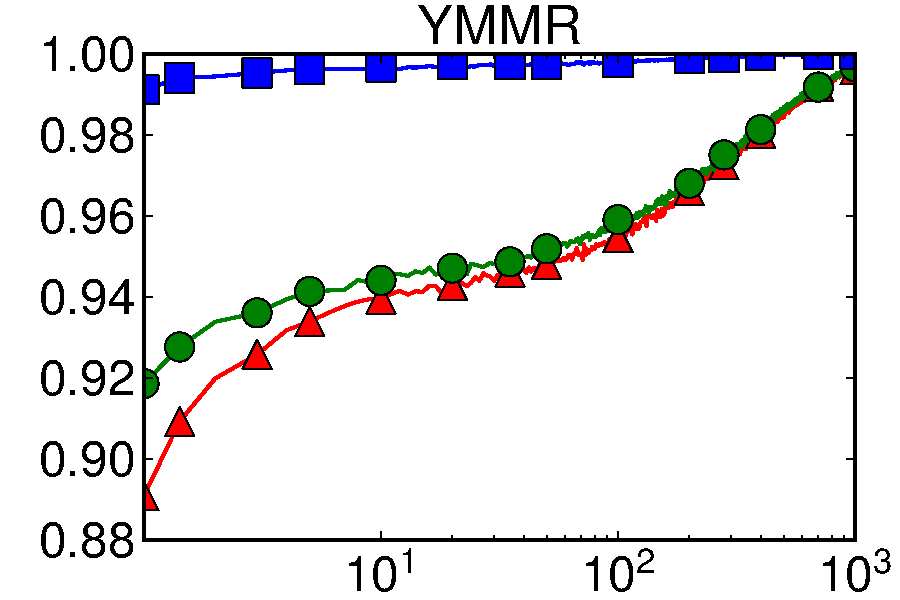
\includegraphics[width=.30\textwidth]{figs/tstales-YMMR.pdf}}\\[-1mm]
\subfigure{
\includegraphics[width=26mm]{figs/stalex.pdf}}
\caption{$(\Delta, p)$-regular semantics for production operation latencies.}
\label{fig:tvis}
\end{figure*}

\vspace{\subsectionskip}\subsection{Quorum Sizing}

In addition to $N$$=$$3$---the most common quorum size we encountered
in practice---we consider how varying the number of replicas (N)
affects $(\Delta, p)$-regular semantics while maintaining
$R$$=$$W$$=$$1$. The results, depicted in Figure~\ref{fig:varyn}, show
that the probability of consistency immediately after write completion
decreases as $N$ increases.  With 2 replicas, \texttt{LNKD-DISK} has a
$57.5\%$ probability of consistent reads immediately after write
completion but only a $21.1\%$ probability with 10 replicas.  However,
at high probabilities ($p$), the window of inconsistency ($\Delta$)
for increased replica sizes is close.  For \texttt{LNKD-DISK},
$\Delta$ at $p=99.9\%$ ranges from $45.3$~ms for 2 replicas to
$53.7$~ms for 10 replicas.

These results imply that maintaining a large number of replicas for
availability or better performance results in a potentially large
impact on consistency immediately after writing. However, the
$(\Delta, p)$-regular semantics probability ($p$) will still rise
quickly (small $\Delta$).

\begin{figure*}[t!]
\centering
\subfigure{
\includegraphics[width=\columnwidth]{figs/nlegend.pdf}}\\[-1mm]
\subfigure{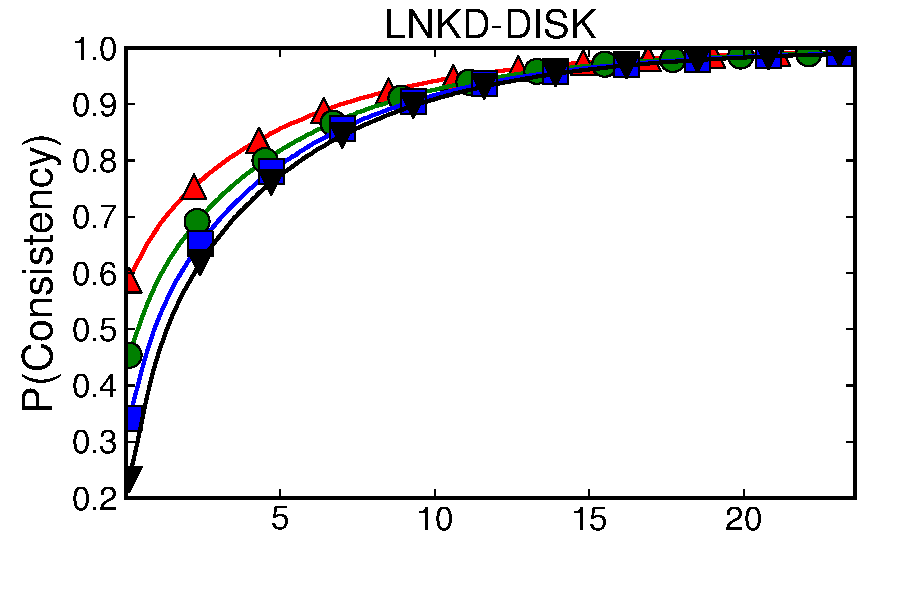
\includegraphics[width=.65\columnwidth]{figs/sweepn-lnkd-disk.pdf}}
\subfigure{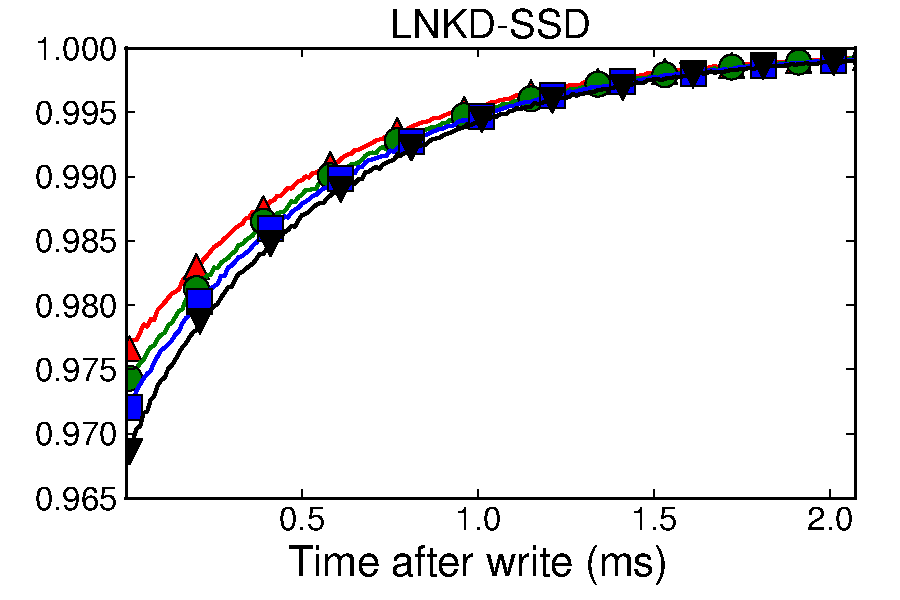
\includegraphics[width=.65\columnwidth]{figs/sweepn-LNKD-SSD.pdf}}
%\subfigure{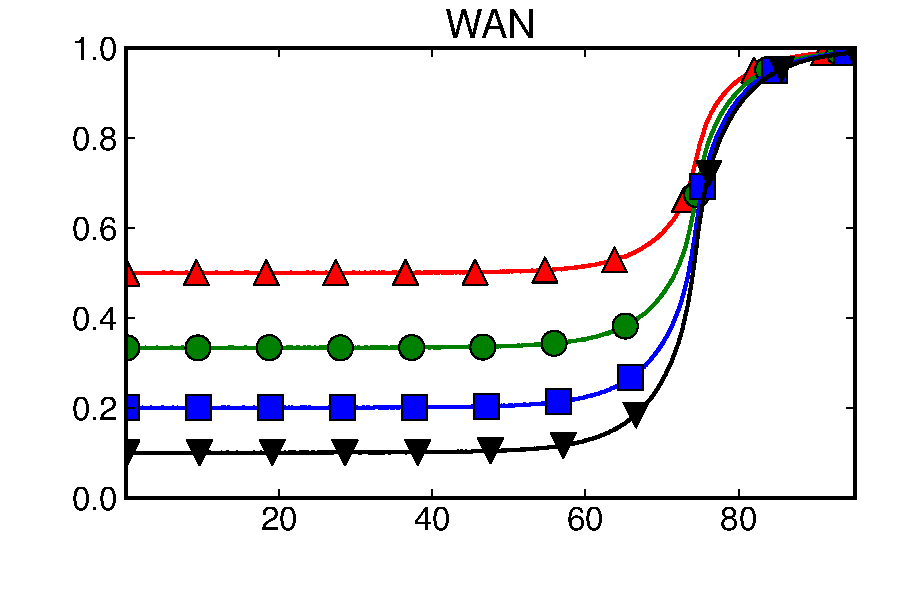
\includegraphics[width=.65\columnwidth]{figs/sweepn-WAN.pdf}}
\caption{$(\Delta, p)$-regular semantics for production operating
  latencies varying the number of replicas $N$ when
  $R$$=$$W$$=$$1$. Inconsistencies $p$ are likely to resolve quickly
  (low $\Delta$) even for large replication factors).}
\label{fig:varyn}
\end{figure*}

\vspace{\subsectionskip}\subsection{Latency vs. Staleness}

Choosing values for $R$ and $W$ is a trade-off between operation
latency and consistency. To measure this trade-off, we compared
$99.9$th percentile operation latencies with the corresponding
$\Delta$ at $p=99.9\%$ for quorum configurations where $N=3$, typical
of deployments in the field.

Partial quorums often exhibit favorable latency-consistency trade-offs
(Table~\ref{table:lat-stale}).  For \texttt{YMMR}, $R$$=$$W$$=$$1$
results in low latency reads and writes ($16.4$~ms) but high $\Delta$
($1364$~ms). However, setting $R$$=$$2$ and $W$$=$$1$ reduces $\Delta$
to $202$~ms and the combined read and write latencies are $81.1\%$
($186.7$~ms) lower than the fastest strict quorum ($W$$=$$1$,
$R$$=$$3$).  Allowing $p=99.9\%$, $\Delta=13.6$~ms reduces
\texttt{LNKD-DISK} read and write latencies by $16.5\%$ ($2.48$~ms).
For \texttt{LNKD-SSD}, across $10M$ writes (``seven nines''), we did
not observe staleness with $R$$=$$2$, $W$$=$$1$.  $R$$=$$W$$=$$1$
reduced latency by $59.5\%$ ($1.94$ms) with a corresponding
$\Delta=1.85$~ms.
% Under \texttt{WAN}, $R > 1$ or $W
% > 1$ results in a large latency increase because writes incur large
% wide-area transit delays. 
In summary, lowering values of $R$ and $W$
can greatly improve operation latency but, even in the tail, the
duration of inconsistency ($\Delta$) is relatively small.

\begin{table*}
\centering
\begin{tabular}{c|c|c|c|c|c|c|c|c|c|}
\cline{2-10}
 & \multicolumn{3}{|c|}{\texttt{LNKD-SSD}} & \multicolumn{3}{|c|}{\texttt{LNKD-DISK}} & \multicolumn{3}{|c|}{\texttt{YMMR}}\\
&\multicolumn{1}{|c}{$L_r$}  & \multicolumn{1}{c}{$L_w$} & \multicolumn{1}{c|}{$t$} &  \multicolumn{1}{|c}{$L_r$} & \multicolumn{1}{c}{$L_w$} & \multicolumn{1}{c|}{$t$} &  \multicolumn{1}{|c}{$L_r$} & \multicolumn{1}{c}{$L_w$} & \multicolumn{1}{c|}{$t$} \\ \hline
\multicolumn{1}{|c|}{$R$$=$$1$, $W$$=$$1$}
&  \textbf{0.66} & \textbf{0.66} & \textbf{1.85} & 0.66 & 10.99 & 45.5 & 5.58 & 10.83 & 1364.0 \\
\multicolumn{1}{|c|}{$R$$=$$1$, $W$$=$$2$}
&  0.66 & 1.63 & 1.79 & 0.65 & 20.97 & 43.3 & 5.61 & 427.12 & 1352.0 \\
\multicolumn{1}{|c|}{$R$$=$$2$, $W$$=$$1$}
& \textbf{1.63} & \textbf{0.65} & \textbf{0} & \textbf{1.63} & \textbf{10.9} & \textbf{13.6}& \textbf{32.6} & \textbf{10.73} & \textbf{202.0}\\
\multicolumn{1}{|c|}{$R$$=$$2$, $W$$=$$2$}
&  \textbf{1.62} & \textbf{1.64} & \textbf{0} & 1.64 & 20.96 & 0& 33.18 & 428.11 & 0 \\
\multicolumn{1}{|c|}{$R$$=$$3$, $W$$=$$1$}
&  4.14 & 0.65 & 0 & \textbf{4.12} & \textbf{10.89} & \textbf{0} & \textbf{219.27} & \textbf{10.79} & \textbf{0} \\
\multicolumn{1}{|c|}{$R$$=$$1$, $W$$=$$3$}
& 0.65 & 4.09 & 0 & 0.65 & 112.65 & 0& 5.63 & 1870.86 & 0 \\
\hline
\end{tabular}
\caption{$\Delta$ for $(p=99.9\%, \Delta)$-regular semantics for
  ($99.9\%$ probability of consistency for $50,000$ reads and writes)
  and $99.9$th percentile read ($L_r$) and write latencies ($L_w$)
  across $R$ and $W$, $N$$=$$3$ ($1M$ reads and writes). Significant
  latency-staleness trade-offs are in bold.}
\label{table:lat-stale}
\end{table*}

We have also experimented with heterogeneous replica behavior and with
multi-item guarantees such as causal consistency and transactional
atomicity. We report results in~\cite{pbs-vldbj}.

\section{Discussion and Future Work}
\label{sec:discussion}

\textbf{Prediction and Verification} In this work, we have developed
techniques for consistency prediction, which provide an expectation of
system behavior given a set of input data about the system and the
current operating environment. Given a trace, one can predict
staleness after an arbitrary amount of time or number of versions
without having to actually run any additional queries. Additionally,
predictions allow users to easily perform ``what-if'' analysis across
arbitrary replication configurations, request distributions ($\Delta$
and $K$), and hardware configurations (e.g., switching from SSDs to
disks). We have found that prediction is computationally inexpensive
and can be performed on a decentralized, per-replica basis. While
prediction is flexible, it is only as good as the input traces. With
representative input data, predictions will be accurate. However, with
unrepresentative data (or bad models), prediction accuracy will
suffer.

In contrast, verification~\cite{rahman2012toward} informs users how
their data stores are performing with guaranteed certainty. If a user
makes a change to their replication settings using a predictor, she
may want to ensure that the change behaves as expected. While this
verification is not well-suited to ``what-if'' analysis, it is an
important complement to prediction. Verification effectively provides
a metric that results from integrating the $(K, \Delta, p)$-regular
semantics PDF weighted by the given read request rate (measured with
respect to time since the last write). Additionally, verification is
algorithmically complex~\cite{podc-hpl}, but, in our experience
is not terribly difficult to implement.

We believe that both techniques will be increasingly useful
as systems begin to treat consistency as a continuous, quantitative
metric.  Taken together, consistency prediction and verification
techniques form a powerful toolkit.

\textbf{White and black box approaches.} In this work, we use a white
box approach to consistency and exploit expert knowledge of
replication protocols to provide quantitative insight. This requires
translating from user-centric, declarative specifications of
consistency anomalies into back-end protocol events (e.g., in the
\textit{WARS} model, the reordering between read and write
responses). We could have alternatively attempted to reverse-engineer
system internals or provide an implementation-independent predictor,
but this black box analysis would be substantially more complex. We
believe that verification techniques are more amenable to black box
techniques and that the portability benefits of black box techniques
must be weighed against their potential inaccuracy. Given our
experiences integrating prediction into existing data stores and the
large-scale adoption of open source data stores, we believe that white
box techniques are feasible, even if they require modifications to
existing stores.

\textbf{Real-world store integration.} With the help of several
open-source developers, we have developed patches for PBS
functionality within two NoSQL stores: Cassandra and Voldemort. For
Cassandra, we have taken two approaches: an invasive but more accurate
implementation and an external but less accurate prediction
module. For the former approach, we modified the Cassandra messaging
layer to add a message creation timestamp in order to measure each of
the \texttt{W}, \texttt{A}, \texttt{R}, \texttt{S} distributions. When
tracing is enabled on a given server, the messaging layer logs
per-operation timestamps in a separate PBS prediction module. The
timestamps are stored in an in-memory circular buffer for each of the
required message latencies.  Subsequently, users can call the PBS
predictor module via an externally accessible interface, which they
can use to provide advanced functionality like dynamic replication
configuration and monitoring (see below). This provides relatively
accurate predictions at the expense of having to instrument the
messaging layer. However, as data stores like Cassandra have expanded
their user-accessible monitoring data (e.g., per-query latency
tracing), we have more recently been exploring predictions outside of
the database---the latter approach---which we have implemented for
Voldemort. We have open-sourced implementations of both approaches.

\textbf{PBS Applications.} PBS enables functionality not possible
without quantitative consistency metrics. With PBS, we can
automatically configure replication parameters by optimizing operation
latency given constraints on staleness and minimum durability.  Data
store operators can subsequently provide service level agreements to
applications and quantitatively describe latency-staleness trade-offs
to users.  Operators can dynamically configure replication using
online latency measurements. This optimization also allows
disentanglement of replication for durability from replication for
reasons of low latency and higher capacity.  For example, operators
can specify a minimum replication factor for durability and
availability but can also automatically increase $N$, decreasing tail
latency for fixed $R$ and $W$. We expanded upon these possibilities in
a SIGMOD 2013 demo that featured real-time predictions for a live
Cassandra cluster and mock web service~\cite{pbs-sigmod}.

\vspace{.5em}
\noindent \textbf{\textit{WARS} limitations and extensions.} There are
several limitations and potential extensions of the \textit{WARS}
model, which we sketch here and discuss in greater detail in extended
versions of this work~\cite{pbs-vldb, pbs-vldbj}. \textit{WARS} only
models a single write and read and is therefore a conservative
estimate for multi-write scenarios. Moreover, in our current
treatment, \textit{WARS} treats each distribution as IID. This is not
fundamental to the model but is a limitation of our latency traces
from industry. \textit{WARS} also does not capture effects of
additional, commonly-employed anti-entropy processes (e.g.,
read-repair, Merkle-tree exchange) and may be a conservative estimate
of staleness. It does not address system behavior under failures,
which varies from store to store, and it assumes that clients contact
a coordinator server instead of issuing requests themselves (e.g.,
Voldemort). We believe that these limitations are not fundamental and
can be accounted for in a white box model but nonetheless remain
future work. Finally, clients requiring staleness detection may do so
asynchronously, enabling speculative reads and compensatory
actions~\cite{pbs-vldb, pbs-vldbj}.

\vspace{\sectionskip}\section{Related Work}
\label{sec:relatedwork}

This research builds upon several related areas: quorum replication, 
consistency models and approaches to quantifying consistency.

Maintaining replicated data is a long-studied problem
in distributed systems and concurrent programming. There is a plethora
of consistency models offering different trade-offs between semantics,
performance, and availability. Traditional models like serializability
and linearizability as well as more recently proposed models such as
timeline consistency~\cite{pnuts} and parallel snapshot
isolation~\cite{walter} all provide ``strong'' semantics at the cost
of high availability, or the ability to provide ``always-on'' response
behavior at all replicas. In contrast, faced with a requirement for
high availability and low latency, many production data stores have
turned to weaker semantics to provide availability in the face of
network partitions~\cite{consistency-partitioning,vogels-defs}.

Our focus in this paper is on the semantics provided by existing,
widely deployed systems. Due to the prevalence of ``strong''
consistency and eventual consistency models in practice (and the
explicit choice between these two models in Dynamo-style systems), we
largely focus on this dichotomy. However, there are a range of
alternative but still ``weak'' models. As an example, the Bayou system
provided a range of ``session guarantees,'' including read-your-writes
and monotonic reads consistency~\cite{sessionguarantees}. Similarly, a
recent Technical Report from UT Austin claims that a variant of causal
consistency is the strongest consistency model achievable in an
available, one-way convergent (eventually consistent)
system~\cite{rtc-proof}, a model that has recently attracted systems
implementations~\cite{eiger}. As we have hinted, probabilistic
approaches are applicable to the consistency models beyond those we
have considered here. Specific to staleness, prior research such as
TACT~\cite{vahdat-article} has examined how to provide deterministic
staleness bounds. These deterministically bounded staleness systems
represent the deterministic dual of PBS.

Our techniques for analyzing modern partial quorum systems draw on
existing, largely theoretical literature. We briefly surveyed quorum
replication~\cite{quorum-overview} in Section~\ref{sec:background}.
In this work, we specifically draw inspiration from probabilistic
quorums~\cite{prob-quorum} in analyzing expanding quorum systems and
their consistency.  We believe that revisiting probabilistic quorum
systems---including non-majority quorum systems such as tree
quorums---in the context of write propagation, anti-entropy, and
Dynamo is a promising area for theoretical work.  While we study
probabilistic guarantees for staleness, prior work on
$k$-quorums~\cite{non-strict,multi-k-quorum} have looked at
\textit{deterministic } guarantees that a partial quorum system will
return values that are within $k$ versions of the most recent
write~\cite{non-strict}.

Finally, recent research has focused on measuring and verifying the
consistency of eventually consistent systems both theoretically and
experimentally (Rahman et al. provide a brief
survey~\cite{rahman2012toward}). This is useful for validating
consistency predictions and understanding staleness violations.

\vspace{\sectionskip}\section{Conclusion}
\label{sec:conclusion}

In this paper, we introduced Probabilistically Bounded Staleness,
which models the expected staleness of data returned by eventually
consistent data stores.  PBS offers an alternative to the
all-or-nothing consistency guarantees of many of today's systems by
offering SLA-style consistency predictions. By extending prior theory
on probabilistic quorum systems, we derived an analytical solution for
the $(K, p)$-regular semantics of a partial quorum system,
representing the expected staleness of a read operation in terms of
versions.  We also analyzed $(\Delta, p)$-regular semantics, or
expected staleness of a read in terms of real time, under Dynamo-style
quorum replication.  To do so, we developed the \textit{WARS} latency
model to explain how message reordering leads to staleness under
Dynamo.  To examine the effect of latency on $(\Delta, p)$-regular
semantics in practice, we used real-world traces from internet
companies to drive a Monte Carlo analysis.  We find that eventually
consistent Dynamo-style quorum configurations are often consistent
after tens of milliseconds due in large part to their resilience to
per-server latency variance. We conclude that eventually consistent
partial quorum replication schemes frequently deliver consistent data
during failure-free operation while offering significant latency
benefits. We believe that continued study and deployment of
quantitative consistency metrics will both enable useful end-user
functionality and shed light on previously opaque and frequently
controversial replication configurations.

\vspace{\sectionskip}\section*{Interactive Demonstration} An
interactive demonstration of Dynamo-style PBS is available at
\url{http://pbs.cs.berkeley.edu/#demo}.

\section*{Acknowledgments}

This work was greatly improved by feedback from many previously noted
individuals~\cite{pbs-vldb, pbs-vldbj}. It was supported by gifts from
Google, SAP, Amazon Web Services, Blue Goji, Cloudera, Ericsson,
General Electric, Hewlett Packard, Huawei, IBM, Intel, MarkLogic,
Microsoft, NEC Labs, NetApp, NTT Multimedia Communications
Laboratories, Oracle, Quanta, Splunk, and VMware.  This material is
based upon work supported by the National Science Foundation Graduate
Research Fellowship under Grant DGE 1106400, National Science
Foundation Grants IIS-0713661, CNS-0722077 and IIS-0803690, NSF CISE
Expeditions award CCF-1139158, the Air Force Office of Scientific
Research Grant FA95500810352, and by DARPA contract FA865011C7136.




% The following two commands are all you need in the
% initial runs of your .tex file to
% produce the bibliography for the citations in your paper.
\scriptsize
\bibliographystyle{abbrv} % standard abbrv style
\bibliography{ernst}  % substitute the name of 'your' Bibliography here
% You must have a proper ".bib" file
% and remember to run:
% latex bibtex latex latex (in that particular order) in order to resolve all the 'numerical values'
% be they for figures, equation numbers, references, footnotes, etc. etc.
%
\balancecolumns
% That's all folks! % GM Sept. 2008
\end{document}
